%%
%%
\chapter{Graph theory}
%%
%%

\section{Warm-up}

In this chapter, we will learn how to represent interactions via graphs.
Let us do so by talking about a question about a city whose existence is of major importance in the history of mathematics -- K\"onigsberg, now part of Russia and known as Kaliningrad.

\begin{figure}[ht]
\centering
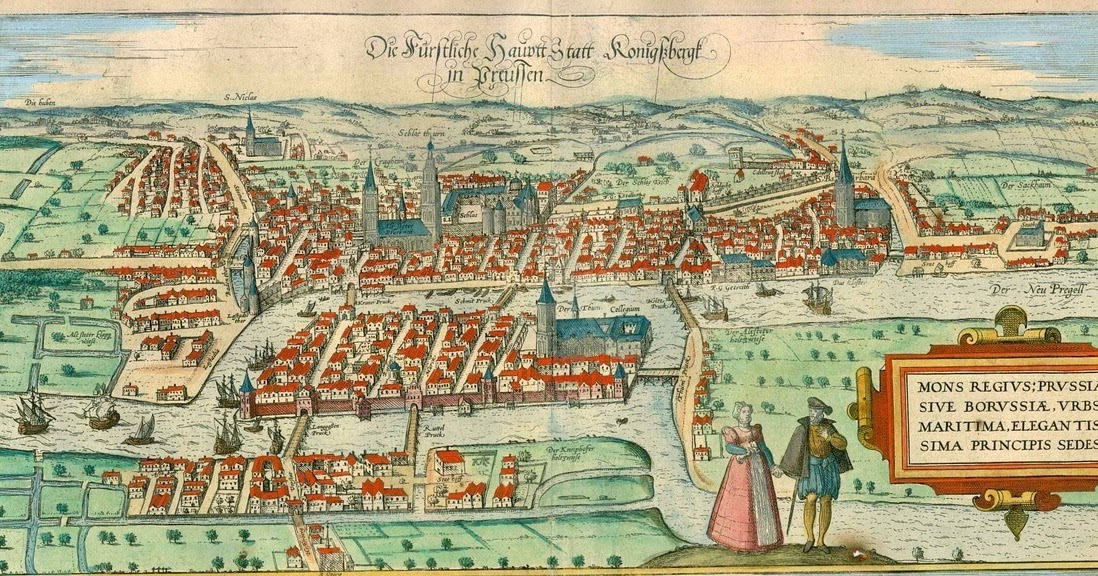
\includegraphics[width=0.4\textwidth]{Figures/Konigsberg.jpg}
\caption{ The map of K\"onigsberg } 
\label{fig:konigsberg}
\end{figure}

Let's highlight the number of bridges in the above map.
Let me give you another picture (copied from the internet) of
the bridges so that you don't have to suffer through the pixelated image.


\begin{figure}[ht]
\centering
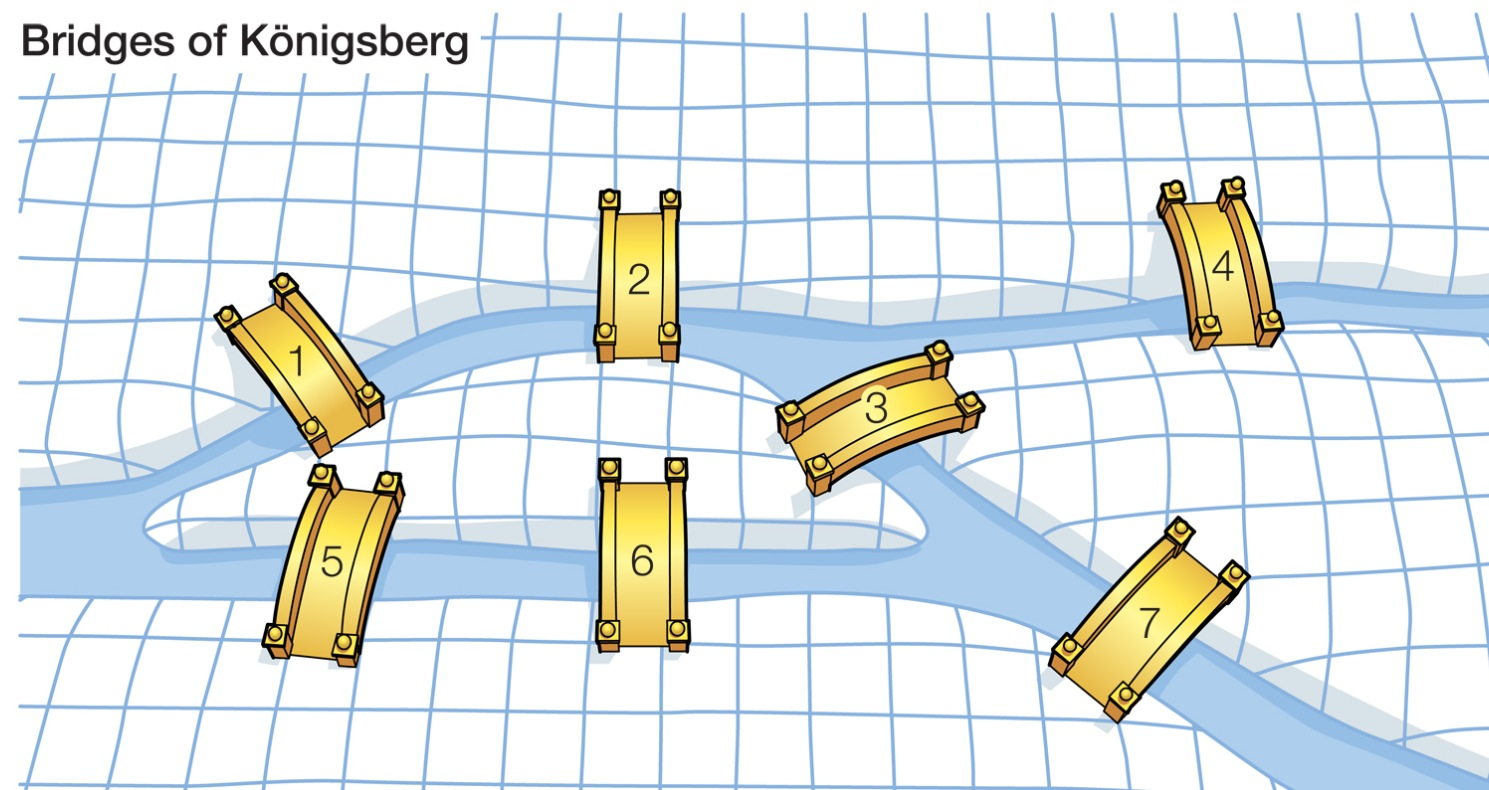
\includegraphics[width=0.4\textwidth]{Figures/Konigsberg-2}
\caption{ Bridges of K\"onigsberg } 
\label{fig:konigsberg-2}
\end{figure}

So you see there are 7 bridges.
According to lore, people in this city would spend Sunday afternoons to walk around
the city and to keep their thoughts occupied, they invented a game: find a path
to walk around the city, crossing each of the bridges only once.
It was an insanely difficult problem as perhaps none of the citizens was able to find a way to do it.

\begin{question}
    Try for 10 minutes to an hour to find a path around the city that crosses each
    bridge only once.
\end{question}

Leonhard Euler, perhaps the most prolific mathematician of all time, was asked this problem and 
thought it had nothing to do with math. But the more he thought about it, the more he was intrigued.
As a result, he invented two fields of mathematics, which are very fundamental to modern world: graph theory and topology.


Before going to talk about the problem, let me give an excerpt from an 
article on the Mathematical Association of America.
\footnote{
\url{https://www.maa.org/press/periodicals/convergence/leonard-eulers-solution-to-the-konigsberg-bridge-problem}
}

\begin{displayquote}
   Why would Euler concern himself with a problem so unrelated to the field of mathematics?  Why would such a great mathematician spend a great deal of time with a trivial problem like the Königsberg Bridge Problem?  Euler was obviously a busy man, publishing more than 500 books and papers during his lifetime.  In 1775 alone, he wrote an average of one mathematical paper per week, and during his lifetime he wrote on a variety of topics besides mathematics including mechanics, optics, astronomy, navigation, and hydrodynamics.  It is not surprising that Euler felt this problem was trivial, stating in a 1736 letter to Carl Leonhard Gottlieb Ehler, mayor of Danzig, who asked him for a solution to the problem:

    ``. . .  Thus you see, most noble Sir, how this type of solution bears little relationship to mathematics, and I do not understand why you expect a mathematician to produce it, rather than anyone else, for the solution is based on reason alone, and its discovery does not depend on any mathematical principle.  Because of this, I do not know why even questions which bear so little relationship to mathematics are solved more quickly by mathematicians than by others.''

Even though Euler found the problem trivial, he was still intrigued by it.  In a letter written the same year to Giovanni Marinoni, an Italian mathematician and engineer, Euler said,

    ``This question is so banal, but seemed to me worthy of attention in that [neither] geometry, nor algebra, nor even the art of counting was sufficient to solve it.''

Euler believed this problem was related to a topic that Gottfried Wilhelm Leibniz had once discussed and longed to work with, something Leibniz referred to as geometria situs, or geometry of position.  This so-called geometry of position is what is now called graph theory, which Euler introduces and utilizes while solving this famous problem. 
\end{displayquote}

I hope you tried the problem out for a good ten minutes. 
It's worth trying to think about the problem as you will have a feel of what's going on
and experience the historic walk in a  city with changed name.
It is not a conincidence that the citizens of K\"onigsberg tried for a long time
and did not succeed. It is impossible to find such a path!

Euler, as clever as he was, realized that usual ways of mathematical thinking
will not solve this problem.
He then, out of thin air, invented an entirely new way to think about it and proved that it is impossible to solve this problem, settling the game for the citizens (which means they will have to invent a new game to play...).
Let's see how he did it!

The following solution is copied from the book~\cite{Burger2013} as the argument 
there  is a direct application 
to Euler's abstract thinking without any abstract theorem.

\begin{proof}[Solution to the K\"onigsberg problem~\cite{Burger2013}]
   The shapes of the landmasses don't matter either, so we can simply replace each landmass by a dot. In fact, the only relevant features are the connections between the landmasses. That is, we focus on which landmass is connected to which other one by a bridge. Each bridge creates a connection between two landmasses.




\begin{figure}[h]
\centering
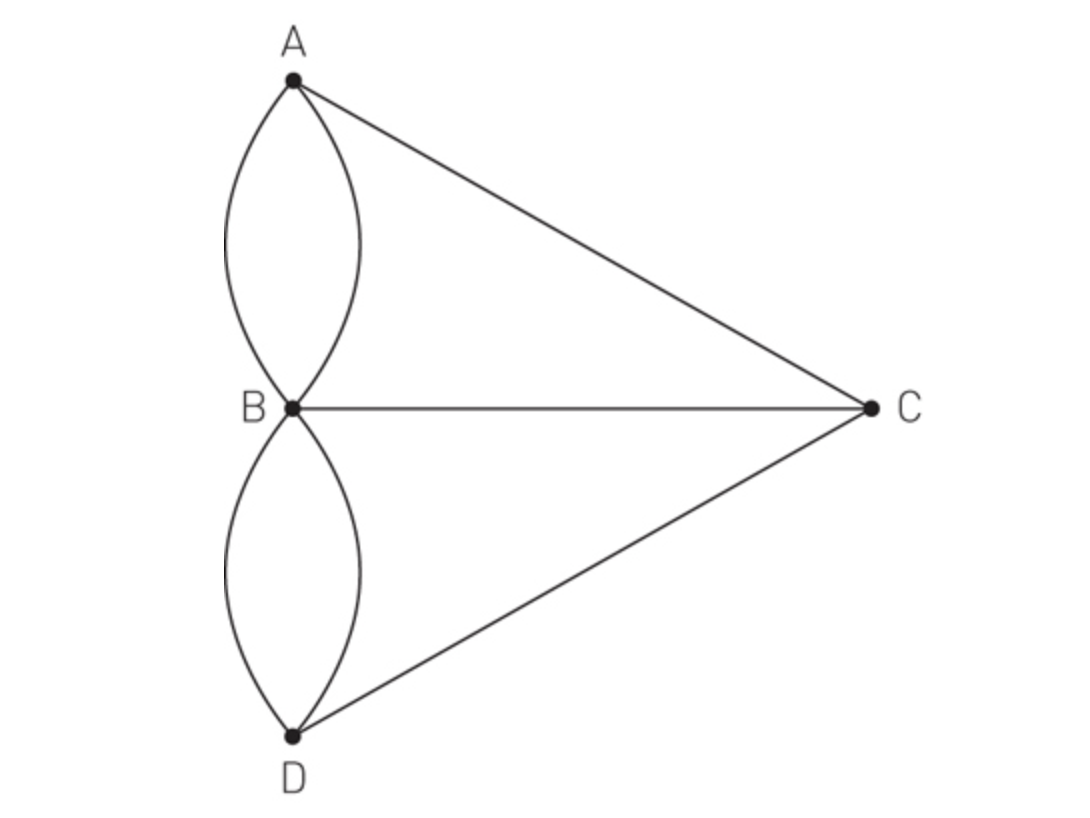
\includegraphics[width=0.4\textwidth]{Figures/Konigsberg-graph}
\caption{ The map of K\"onigsberg in graph form } 
\label{fig:konigsberg-graph}
\end{figure}

Now we are well on our way to isolating the essential features of the Königsberg Bridge Puzzle. We have a collection of places (landmasses now denoted as dots) and some pairs of them are connected (bridges now denoted as arcs between pairs of dots)—and these places and connections are all that matter for the challenge at hand. We could name the places A, B, C, and D. And we could describe the connecting bridges by writing which pair of places each bridge connects. So the seven bridges of Königsberg can now be denoted as AB, AB, AC, BC, BD, BD, and CD.





After we've stripped away all the unnecessary diversions, we could restate the Königsberg Bridge Puzzle as follows: Suppose we have four dots named A, B, C, and D, and we have seven connections among them, namely, AB, AB, AC, BC, BD, BD, and CD. Can we start at some dot and choose connections to take us from dot to dot in such a way that we use every connection exactly once and we return to the dot at which we started? Notice that the starting place does not matter; that is, if we could solve the puzzle starting at some dot we could also solve it starting from any other dot. Why is this true?

It might, at first, appear that we have not really made any progress toward solving the puzzle, but we have isolated the essential ingredients, and that is an enormous step forward. In fact, those essential ingredients—dots and connections—are the essential ingredients that comprise a modern mathematical area called graph theory. A graph is simply a set of vertices (that is, the dots) together with a collection of connections of pairs of the vertices (that is, the lines or arcs connecting pairs of dots). The connections are called edges. So the graph associated with the Königsberg Bridge Puzzle has vertices A, B, C, and D and edges AB, AB, AC, BC, BD, BD, and CD. Our simple picture that just shows the vertices and edges has all the information we require to tackle the Königsberg Bridge Puzzle. Now we can restate the Königsberg Bridge Puzzle as follows: Can we start at some vertex in the Königsberg graph, then choose edges to take us from vertex to vertex in such a way that we use every edge exactly once and we return to the vertex at which we started?

The Königsberg graph shows us that there are four landmasses (represented by the vertices) and it shows which landmasses are connected by bridges (represented by the edges). By the way, the order of the vertices that describe an edge does not matter; in other words, CD and DC both mean the same thing, namely, a “bridge” (or edge) connecting landmasses C and D. Since two bridges connect A to B and two bridges connect B to D, we simply list AB twice and BD twice, but we don't make any attempt to distinguish the two AB bridges from one another. For example, we don't care which AB is the bridge nearer D. We make no distinction between the two AB edges, because an edge is just a connection between its vertices. No other feature of an edge matters, such as how or where we draw it.

If we take a walk over the edges of the Königsberg graph, we can represent that walk by the ordered sequence (list) of edges that we traversed. For example, if we just go from A to B to D to C to B and back to A, we could represent that walk by listing the edges (AB)(BD)(DC)(CB)(BA) in the given order. Notice that it doesn't matter which of the two BD edges we choose, as each one accomplishes the same task of getting us from B to D.


Suppose we take a walk around the Königsberg graph and return back to where we started. If we write down the ordered sequence of edges involved, notice that each edge that we traverse must start at the point at which the previous edge ended. So in our example (AB)(BD)(DC)(CB)(BA), after we traveled along one of the edges from A to B, the next edge of course started at B and ended at some other point, in this case D. Then we took an edge from D to C, then journeyed on the edge from C to B, and then went from B to A using the edge we didn't use the first time. Since we returned to the place where we started, the first letter and the last letter will coincide.


Let's forget the parentheses and just look at the letters that are written down in our list of the edge-sequence, namely, ABBDDCCBBA. Notice that every letter appears an even number of times, because every internal letter is the end of one edge and therefore, in turn, the beginning of the next edge, so every internal letter appears in pairs, while the first and last letters are the same (because we return to where we started), so that letter appears in pairs as well. 
The list of edges of such a circuit is the Noah's Ark of graph theory: Every letter appearing comes in pairs, in this example: BB, DD, CC, BB, and of course our starting and ending location AA.

This observation about letters appearing an even number of times lets us solve the Königsberg Graph Puzzle. Why? Well, let's look at the list of all seven edges of Königsberg. They are AB, AB, AC, BC, BD, BD, CD. If we walked over all the Königsberg edges each exactly once in any order at all, those seven pairs of letters would be the ones describing our walk. It might start (AB)(BC)(CD)… and so on. But if each edge in the Königsberg graph (that is, each given pair of letters such as AC) appeared exactly once in our walk, then the total number of A's would be 3 (an odd number), because we can see that there are exactly three A's in our seven edges—namely one A each in the edges AB, AB, and AC, and no other A's in any of the other edges. Similarly, the total number of B's would be 5, the number of C's would be 3, and the number of D's would be 3.

But we saw that if we were able to take a walk over the edges—traversing each edge exactly once—and return to where we started, then when we recorded the edges in the order that we walked over them, each letter would appear an even number of times. But this even number of appearances of each letter is impossible for the Königsberg graph because we just noticed that each letter appears an odd number of times on our list of bridges. Thus we conclude that it is impossible to start at one location, traverse each and every edge exactly once, and return to our starting point.

This observation settles the Königsberg Graph Puzzle and thus settles the Königsberg Bridge Puzzle, definitely proving that it is impossible to walk over each bridge just one time. Please think through the reasoning and “bridge” the ideas of the argument together for yourself until every step makes sense.
\end{proof}

\section{Graph theory}

Let us recap some essential ideas in the above argument 
and turn them into mathematical symbols.
\begin{definition}[Graph]
    A \emph{graph} $G = (V,E)$ consists of a set $V$ of \emph{vertices} (or \emph{nodes})    
    and a set $E$ of \emph{edges}.
    
    An \emph{edge} in a graph is a curve that has endpoints connecting a vertex to another 
    vertex or a vertex to itself.
    
    A \emph{loop} in a graph is a curve that connects a vertex to itself.
\end{definition}

There are various ways to represent vertices and edges. One way is just to draw out
the graph as in Figure~\ref{fig:konigsberg-graph}.
Another way is to just write down the list of vertices in a set such as
\begin{equation*}
    \set{A,B,C,\dots} \,,
\end{equation*}
and a list of edges and loops connecting the vertices by writing the vertices next to each other such as
\begin{equation*}
    \set{AB, AA, BC, BA, \dots} \,.
\end{equation*}

\begin{definition}[Path]
    A \emph{path} is a succession of edges of the form $v_1v_2,v_2v_3,\dots, v_n v_{n+1}$ so that
    all the edges and vertices only appear once when drawn out.
\end{definition}
\begin{definition}[Connected graph]
    A graph $G = (V,E)$ is called \emph{connected} if, for any pair of vertices $A, B \in V$, there is a path from $A$ to $B$.
\end{definition}


\begin{definition}[Eulerian path]
    An \emph{Eulerian path} is a path through a graph which traverses each 
    edge exactly once.
\end{definition}

\begin{definition}[Eulerian cycle]
    An \emph{Eulerian cycle} is an Eulerian path that ends in the same vertex where it started.
\end{definition}


\begin{definition}[Degree]
    In a graph $G = (V,E)$, the \emph{degree} of a vertex $A$, denoted by $\deg(A)$
    is the number
    of edges that connect to $A$, and loops (i.e. edges $AA$) are counted twice. 
\end{definition}




\begin{theorem}
    Let $G$ be a finite connected graph. Then an Eulerian path exists if and only if there are at most two vertices with odd degree, and if there are, vertices of odd degrees must be the start or the end of the path. An Eulerian cycle exists if and only if all vertices have even degrees.
\end{theorem}






%%%
\section{Coloring maps and what graphs have to do with it}
%%%

%%%
\subsection{Motivation}

\paragraph{Acknowledgement:} This lecture is based on material shared by Renee Bell and Patrick Shields.

\begin{question}
    If you take a world atlas and pick a region, what is the minimal number of colors you would need to color every country in a way that each pair of countries that share a borderline has different colors?
\end{question}

You can try, unsuccessfully, to color Central America with two colors. Try it and notice how you run into trouble around the point where three countries come together, for example Mexico, Belize and Guatemala:

\begin{center}
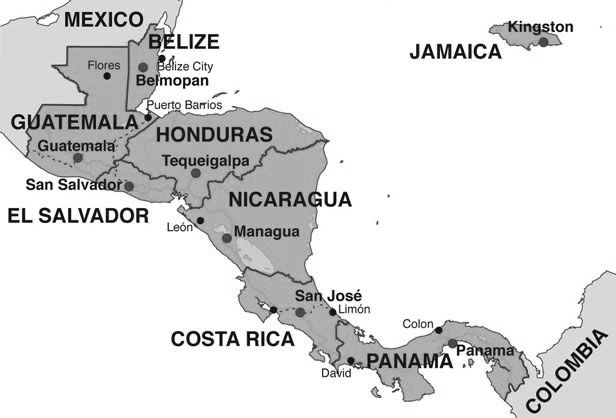
\includegraphics[width=7cm]{pics/central-america-uncolored.jpg}
\end{center}


However, it \textit{is} possible to color this map using three colors:

\begin{center}
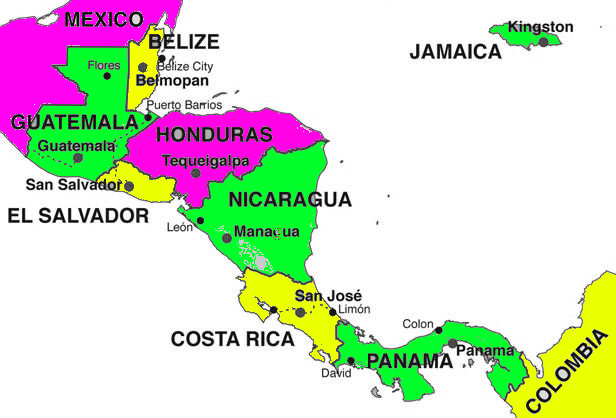
\includegraphics[width=7cm]{pics/central-america-colored.png}
\end{center}


Alright, maybe we can do this for all maps using 3 crayons. Let's consider the following map of the planet of Chromatica, which is in another galaxy, and has countries A,B,C, and D.

\begin{center}
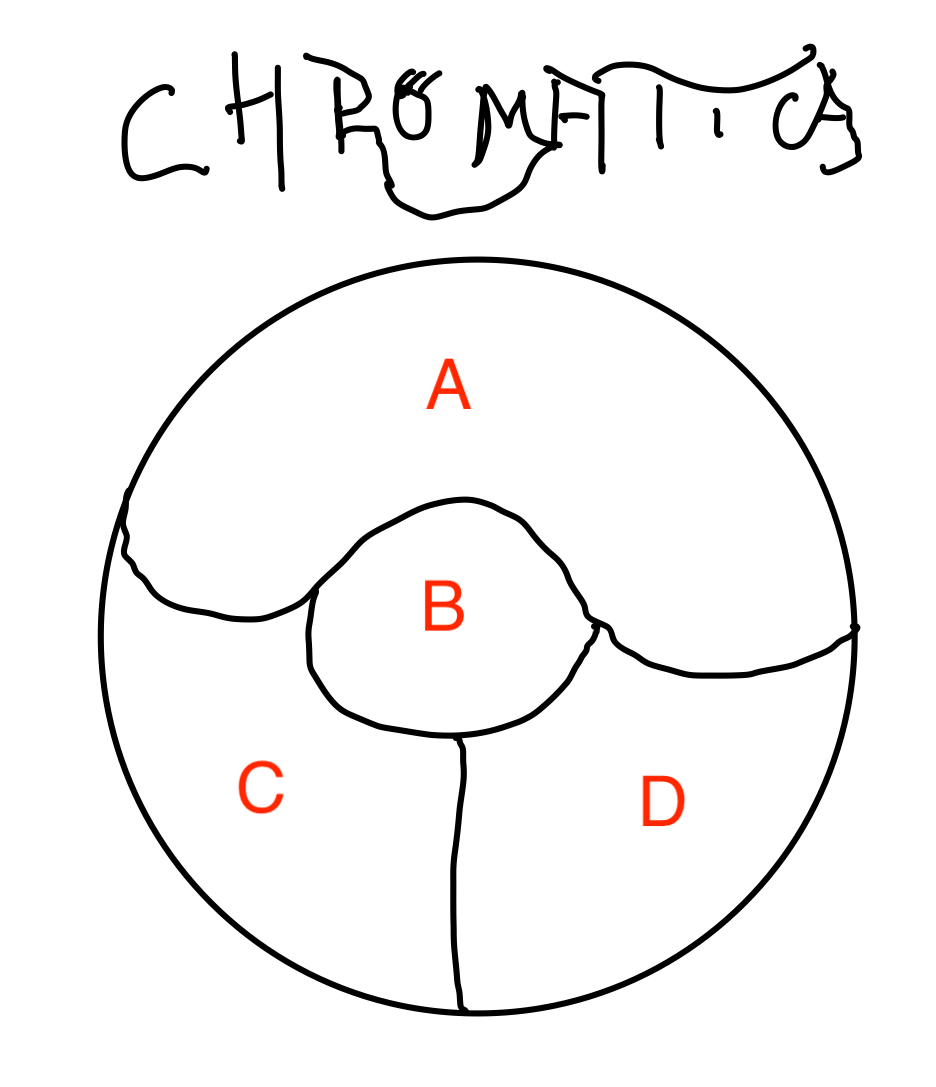
\includegraphics[width=7cm]{pics/chromatica-uncolored.png}
\end{center}

\begin{question}
Can you find a coloring of Chromatica which uses only three colors?
\end{question}

In this case, even three is not enough! If we color A pink, then neither C nor D can be pink, since they're touching A. But C and D cannot be the same color, since C is touching D. So, let's say C is green and D is yellow. Then B is left touching a pink state, a green state, and a yellow state. So it can't be any of those colors. We will need a fourth color, let's say blue.

\begin{center}
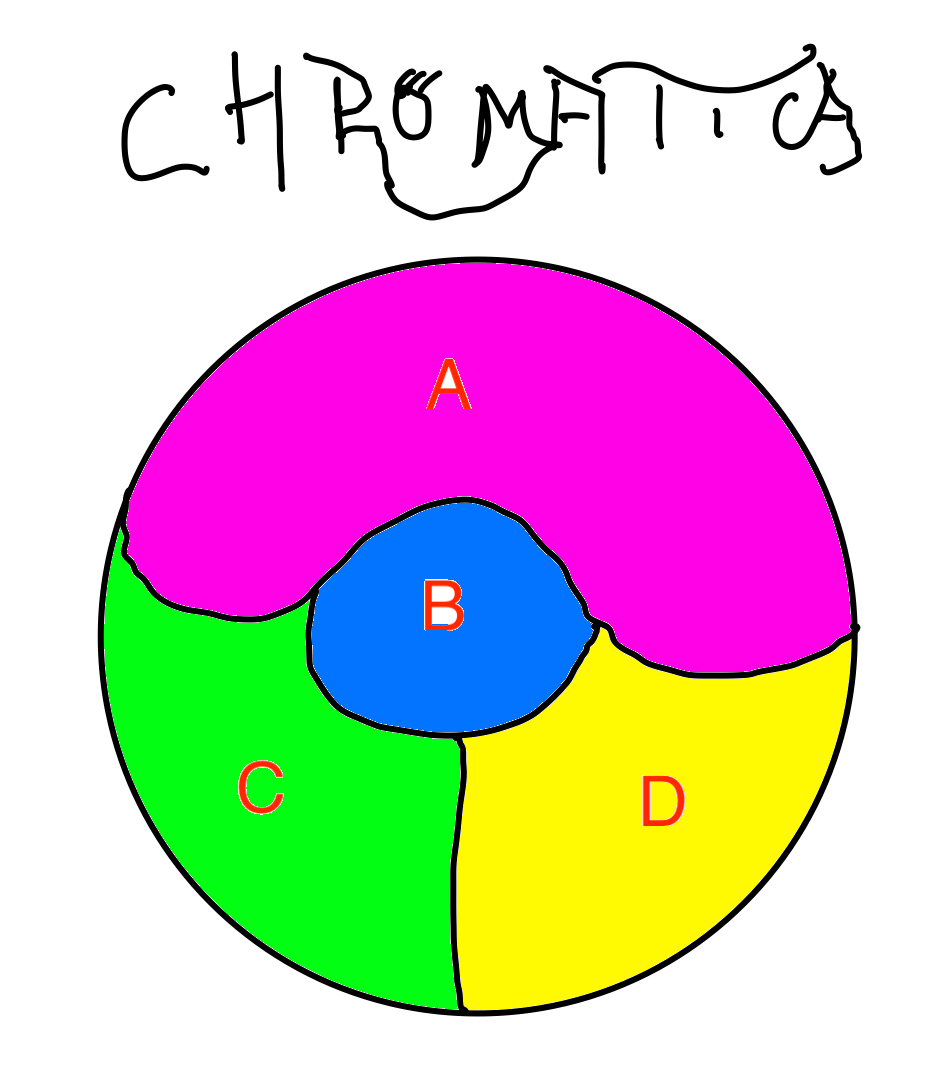
\includegraphics[width=7cm]{pics/chromatica-colored.png}
\end{center}

Could there be a map where even four colors isn't enough?
It turns out the answer is no, but it took a long time to prove that decisively. The conclusive answer to this question was given by Kenneth Appel and Wolfgang Haken in 1976, in the form of the following theorem, called the Four Color Theorem.

\begin{theorem}[Four Color Theorem for Maps]
Every map can be colored such that no two regions which share a boundary are the same color, using four colors.
\end{theorem}


%%%
\subsection{Graphic content}

Now let's try to abstract and simplify this problem, especially for people who are not great at drawing countries.
The only information we needed was which countries share a boundary! So let's record that information using a graph.\\

We create a graph associated to this map, with a vertex for each country and an edge between two vertices if the associated countries share a boundary. Here are the graphs for Central America and Chromatica:

\begin{center}
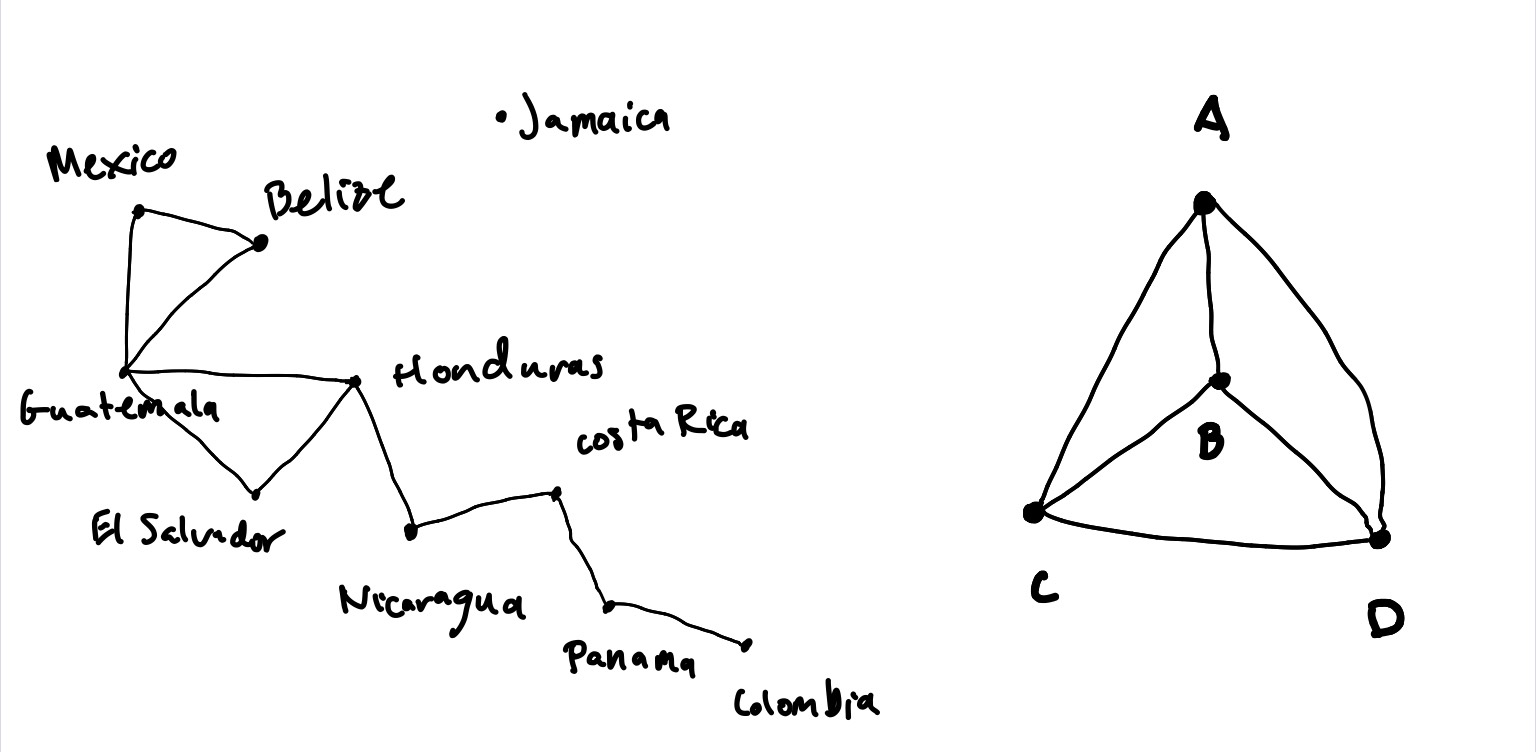
\includegraphics[width=11cm]{pics/map-graphs.jpeg}
\end{center}

Now the question reduces to coloring the \textit{vertices} of these graphs so that no two vertices which share an edge are the same color. Let's formalize this in a definition:

\begin{definition}
A \textbf{coloring} of a graph is a labeling of the graph’s vertices with colors such that no two vertices sharing the same edge have the same color.
\end{definition}

If you don't have a lot of colors at your immediate disposal, you can label colors by numbers, symbols, letters of Japanese alphabets, whatever suits your tastes better.

Here are the colorings of the graphs associated to Central America and Chromatica corresponding to the map colorings we just did:

\begin{center}
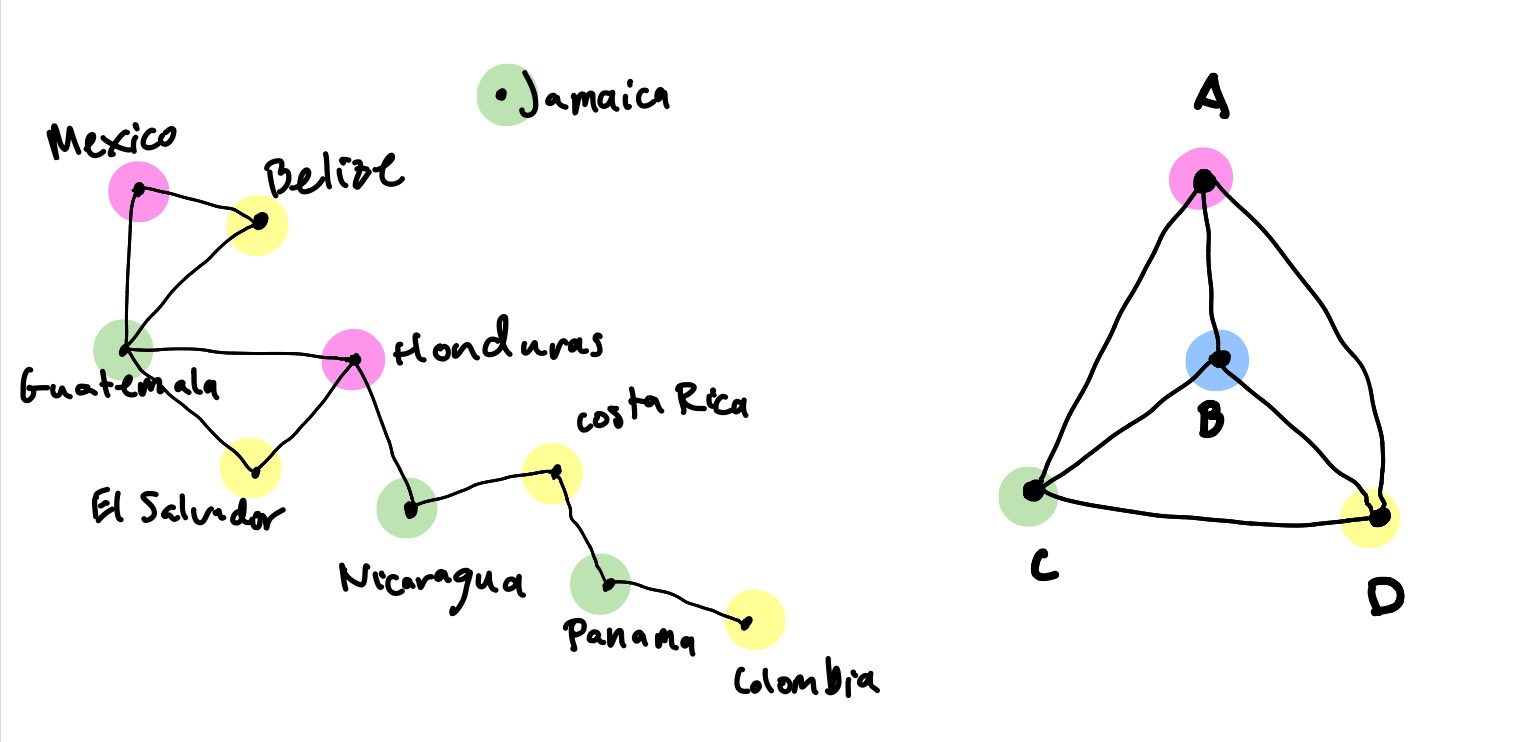
\includegraphics[width=11cm]{pics/map-graphs-colored.jpeg}
\end{center}

We're also trying to figure out the number of colors we need to do this. This motivates the following definition:

\begin{definition}
A coloring using $k$ colors is called a  $k$-\textbf{coloring}. The smallest number of colors needed to color a graph $G$ is called its \textbf{chromatic number}, and is denoted $\chi(G)$.
\end{definition}

In the examples we just saw, $\chi$(Chromatica)$=4$, since we can color it using four colors but NOT using fewer. We also calculated that $\chi$(Central America)$=3$.\\ 

The definitions we just gave could be for any kind of graph. For example, the pentagram, which we will call $P$:

\begin{center}
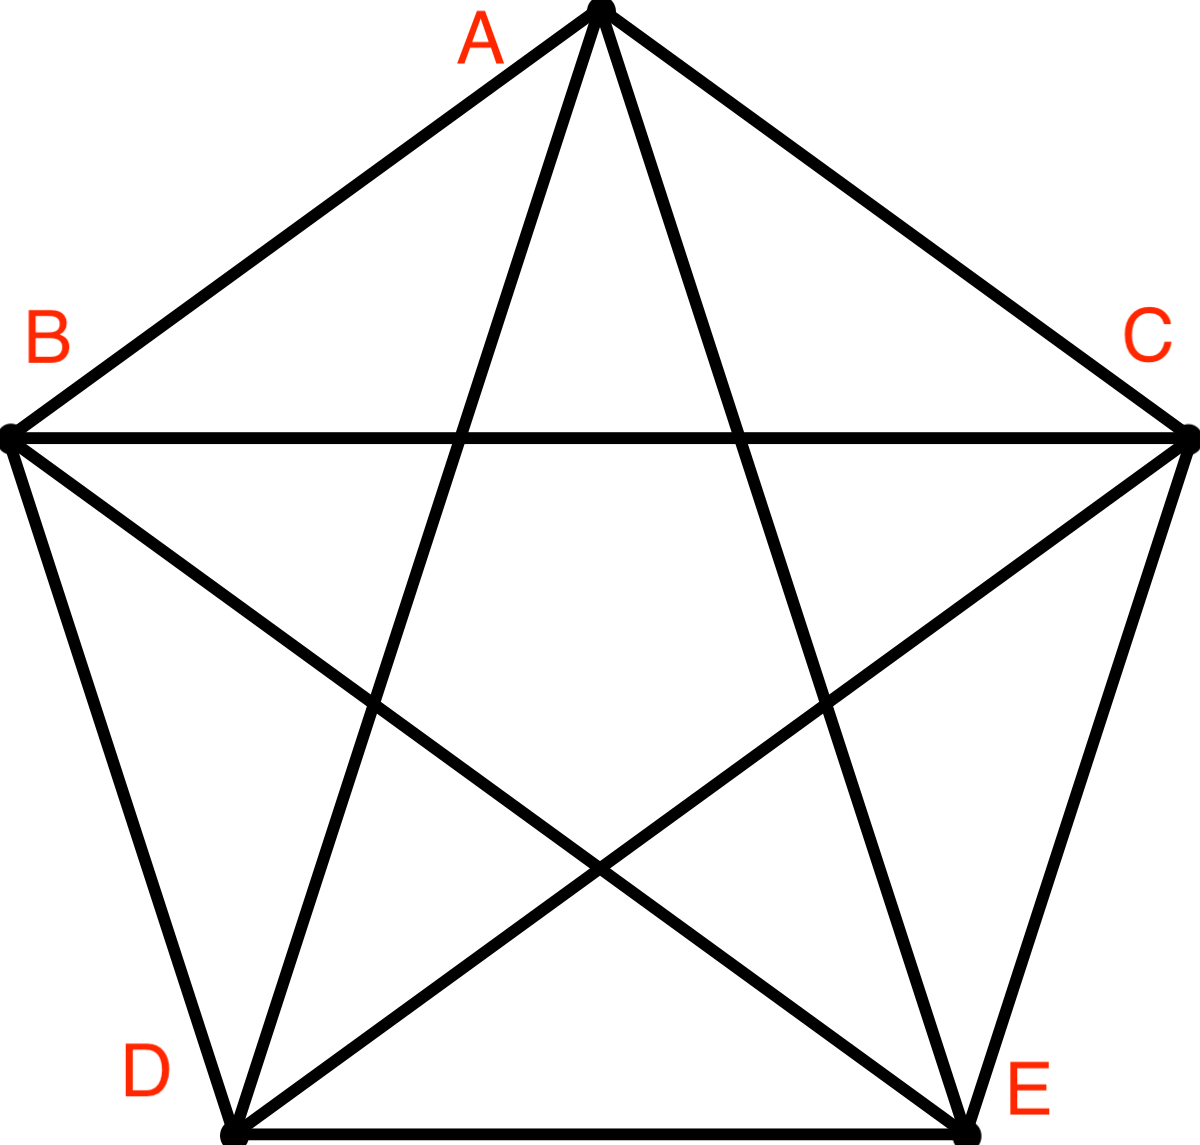
\includegraphics[width=6cm]{pics/Pentagram.png}
\end{center}

Let's calculate its chromatic number. Of course, we could 5-color it by just making every single vertex a different color, so we know $\chi(P) \leq 5$. 
So, can we color it using four colors? Well, let's say we color A ``color 1''. Since B shares an edge with A, it must be a new color, ``color 2''. Since C shares an edge with both A and B, it must be a new color, ``color 3''. D must be a fourth color, ``color 4''. And finally, E touches every other vertex, so it must be a fifth color. $P$ cannot be colored using 4 colors, so $\chi(P) = 5$.\\



But wait, didn't we just say that four colors is enough? Well, that was only for \textit{maps} which are ``2-dimensional'' in some sense, not \textit{all} graphs. The type of graph that we made is called \textbf{planar}.\\

\begin{definition}{}
A graph is \textbf{planar} if it can be drawn on the plane (that is, in two dimensions) in such a way that its edges intersect only at their endpoints.
\end{definition}

We can now give a different version of the Four Color Theorem:

\begin{theorem}[Four Color Theorem for Graphs]
Every planar graph can be 4-colored.
\end{theorem}

Now we see that the problem with the pentagram is that it's not planar; it can't be ``untangled'' into a nice 2D graph that lies flat in the plane.
\\

%%%
\subsection{Conflict Resolution}

I realize that not all of you are planning to become cartographers, but most of us have to deal with conflict sometimes, so let's look at a more likely application.
Suppose you are planning a small dinner, now that the worst of the lockdown is over, and want to determine a seating chart, seating people at different tables.
You are inviting your friends Jane, Matt, Imani, Hyunjeong, Bessam, Padma, and Alejandro. You love them dearly, but they are very... passionate people, and you know that if you seat two of them who disagree at the same table, the dinner is going to go very badly. Here are their conflicts:
\\

Matt and Imani are Patriots fans. Jane and Padma are Eagles fans. 
Do not sit them next to each other! Also, Hyunjeong likes Cardi B but Alejandro and Bessam are hardcore Nicki Minaj stans (barbz), so she won't sit with either of them. Alejandro dated both Matt and Jane so he doesn't want to sit with them, because that would be awkward. Other than that, everyone is cool. Let's list the conflicts:
\begin{enumerate}
    \item Matt can't sit with Jane
    \item Matt can't sit with Padma
    \item Imani can't sit with Jane
    \item Imani can't sit with Padma
    \item Hyunjeong can't sit with Bessam
    \item Hyunjeong can't sit with Alejandro
    \item Alejandro can't sit with Jane
    \item Alejandro can't sit with Matt
\end{enumerate}

We can record this information in the following chart:
\begin{center}
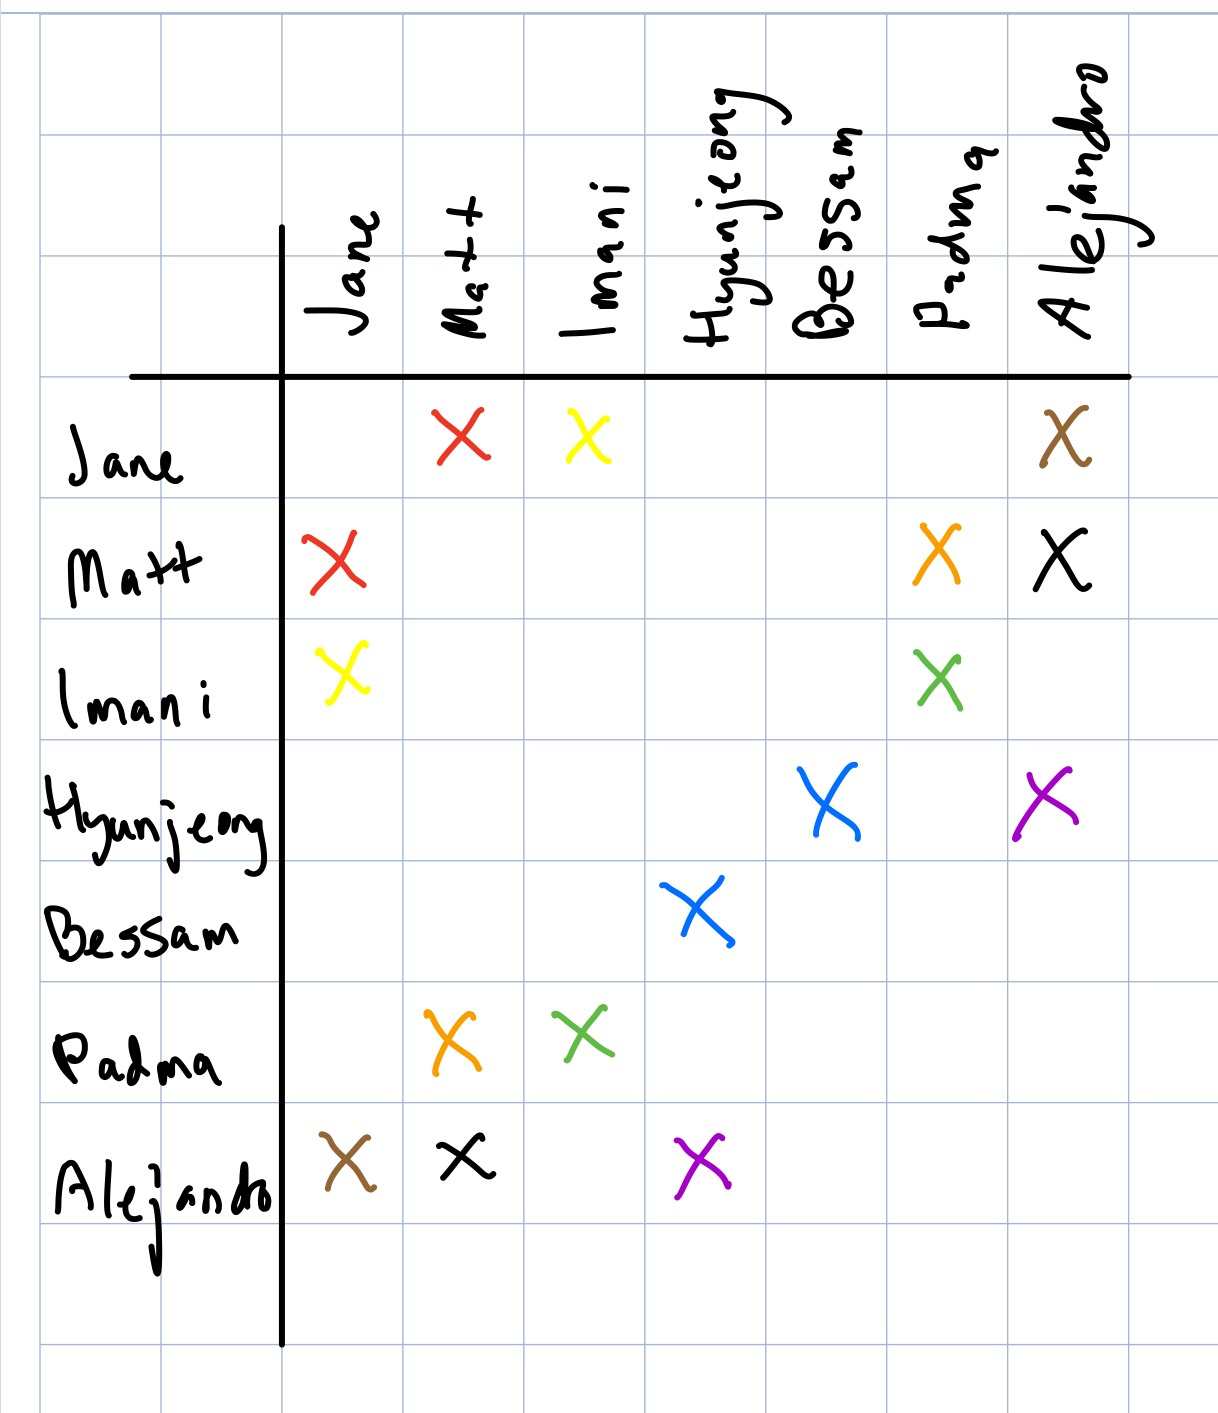
\includegraphics[width=7cm]{pics/dislike-chart.jpeg}
\end{center}

This is a very neat, excel-spreadsheet style way to record the information. But we can also record it in a graph. The only thing that matters for us is whether or not any two people have conflict. So we can create a graph where the vertices represent people, and there is an edge between two people if there is conflict between them.
We show this with the colors corresponding to the conflicts on the left, and in black and white on the right. We will not really need to color the edges, but we will have to color the vertices.

\begin{center}
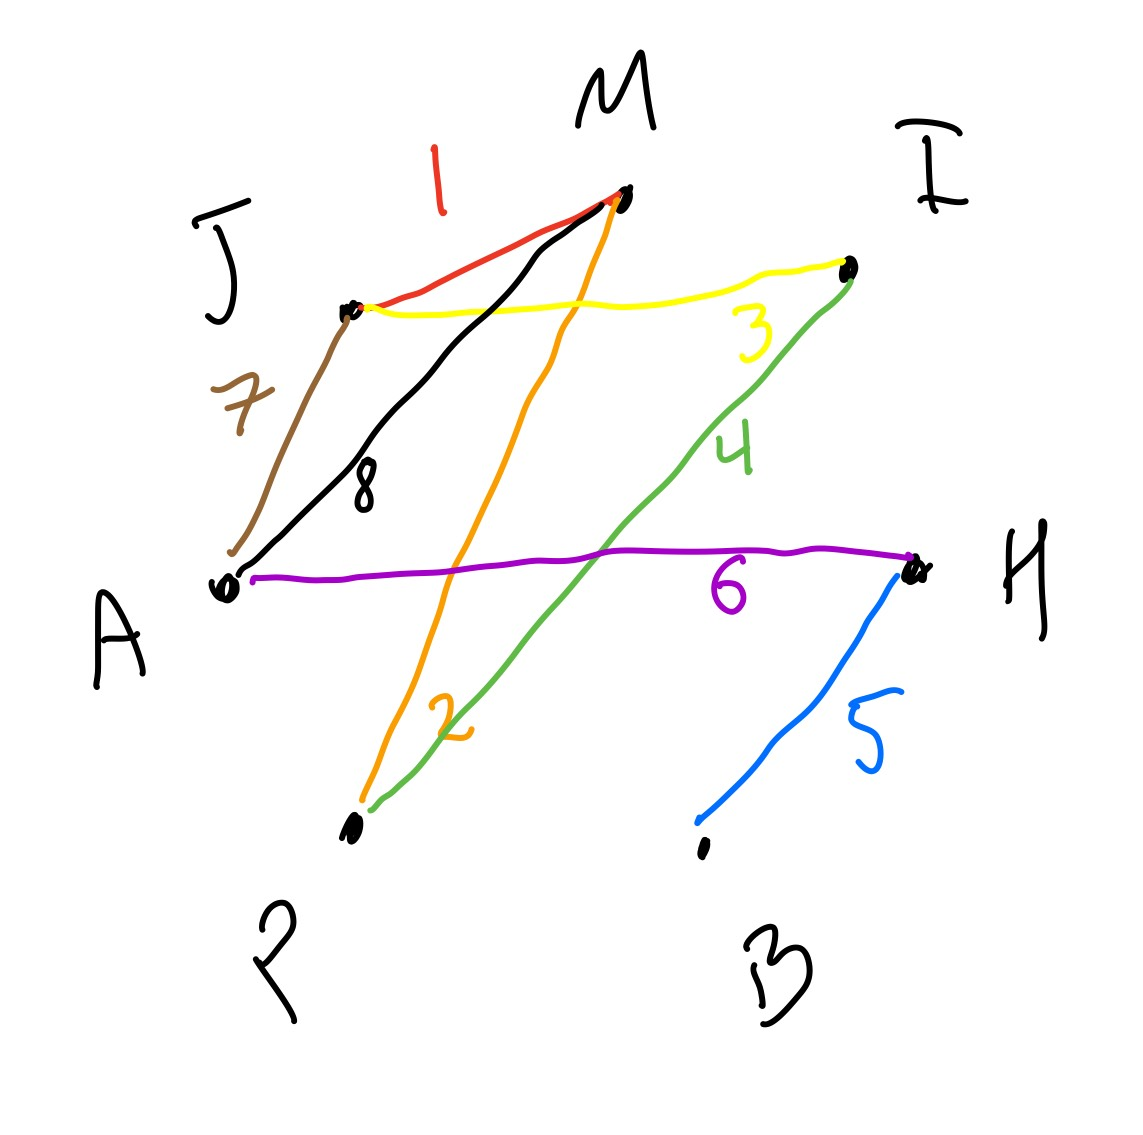
\includegraphics[width=6cm]{pics/conflict-graph.jpeg}
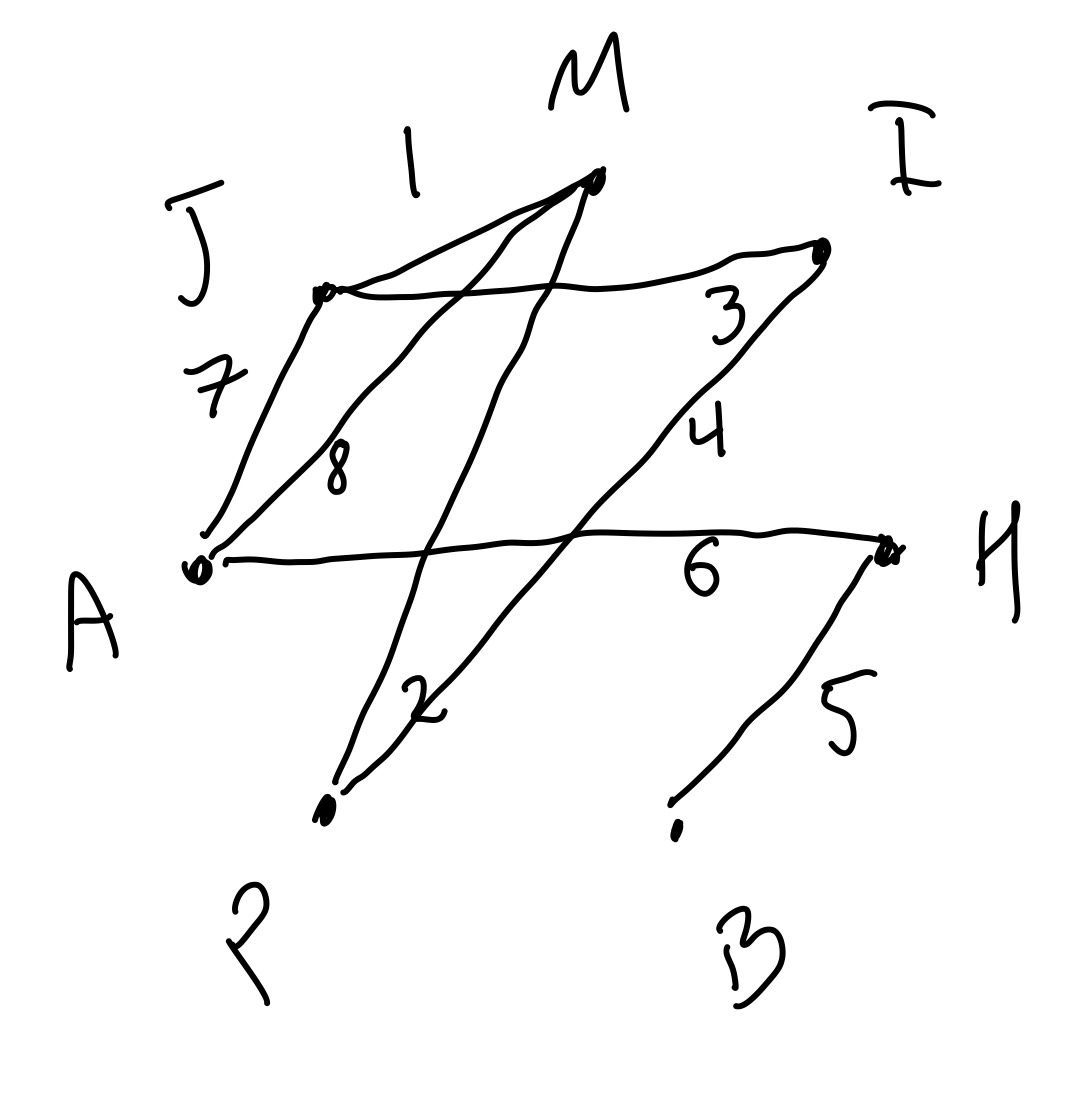
\includegraphics[width=6cm]{pics/conflict-graph-bw.jpeg}
\end{center}

\begin{question}{}
How can you figure out how many tables you will need for your dinner using this graph?
\end{question}

We just learned a new thing we can do with graphs, which is color them. You can think of a coloring using $k$-colors as a way of putting the vertices into $k$ groups, where no group has any two vertices which share an edge. 

Conversely, if we put the vertices into $k$ groups, where no group has any two vertices which share an edge, we can use that to make a $k$-coloring for the graph! We just pick a color for each group, and then color the vertices in each group accordingly.


Back to the dinner; we can find a 3-coloring of the graph using red, yellow, and blue as follows:

\begin{center}
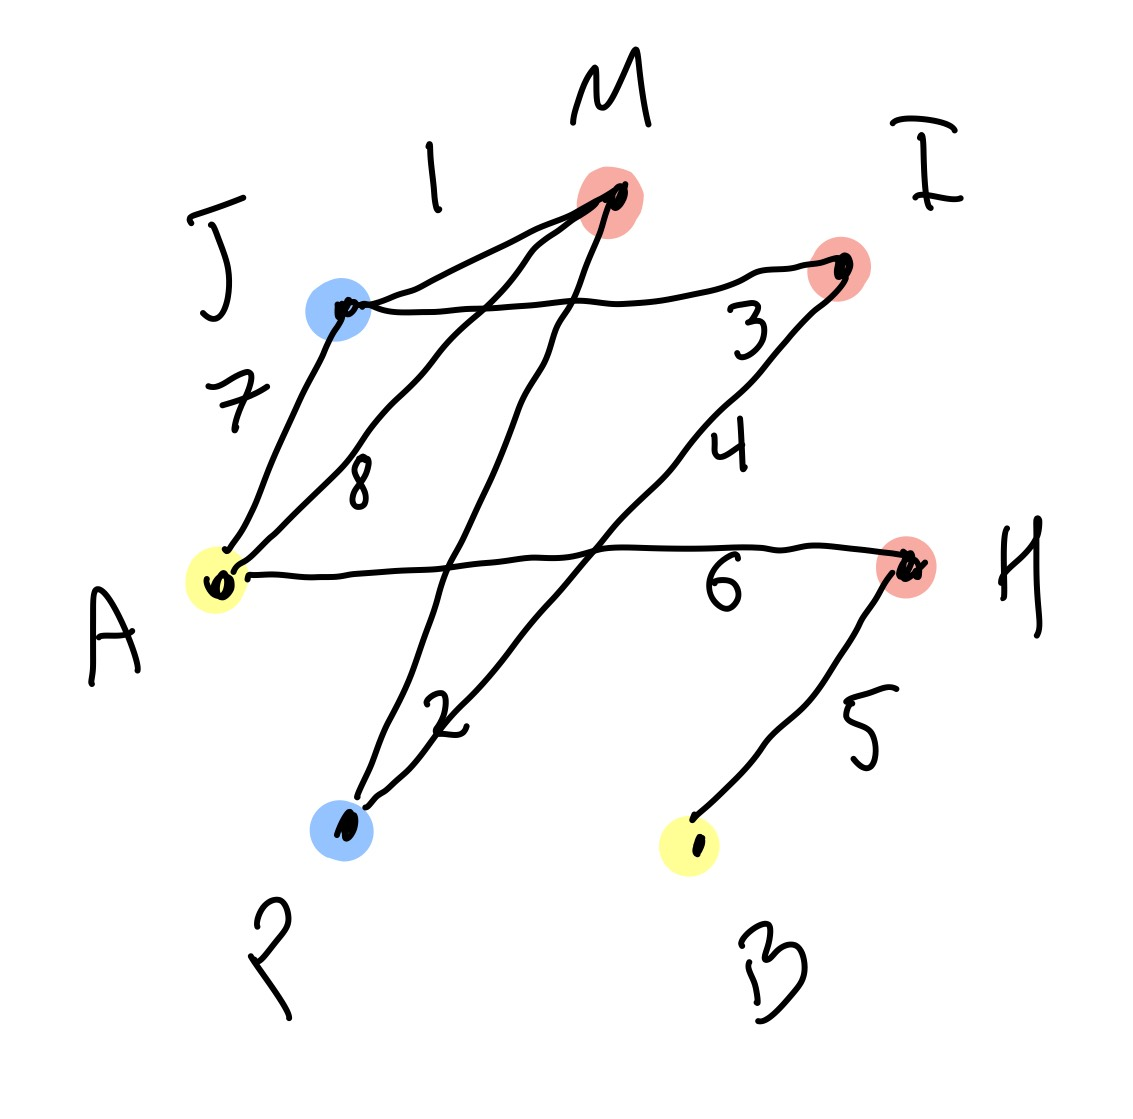
\includegraphics[width=8cm]{pics/conflict-3-colored.jpeg}
\end{center}

This allows us to seat everyone using 3 tables! You can refer to tables as the red table, the yellow table, and the blue table. The graph above corresponds to the following seating:

\begin{center}
\begin{tabular}{c|c}
 \multicolumn{2}{c}{Tables}\\
\hline
 Color & Vertices of that color \\
 \hline
 \hline
 Red & Matt, Imani, Hyunjeong\\
 \hline
  Yellow & Alejandro, Bessam \\
 \hline
  Blue & Jane, Padma \\
 \end{tabular}
 \end{center}
 
 You can check that this graph can't be 2-colored. This means there's no way of seating everyone at 2 tables without there being some conflict. Better bring enough tables!\\
 
\subsection{Scheduling}
Let's look at one \textit{final} application: scheduling final exams. 
Suppose we're scheduling exams for Math, Computer science, French, Sociology, Biology, and Anthropology.
We'll make a graph where the vertices are subjects, and there is an edge between two vertices if the corresponding subjects have a conflict.\\

Suppose that Student 1 is in Math, French, and Sociology.
This means that Math and French are in conflict, French and Sociology are in conflict, and Math and Sociology are in conflict (since this student can't attend both exams at the same time).
So there is an edge between Math and French, an edge between French and Sociology, and an edge between Sociology and Math.


Suppose also that
Student 2 is in Anthropology, French, and Sociology, Student 3 is in Biology and Computer science, Student 4 is in Computer science and Mathematics, and Student 5 is in Math and Anthropology.

This gives rise to the following graph, where the conflict edges are colored according to which Student is the cause of them:

\begin{center}
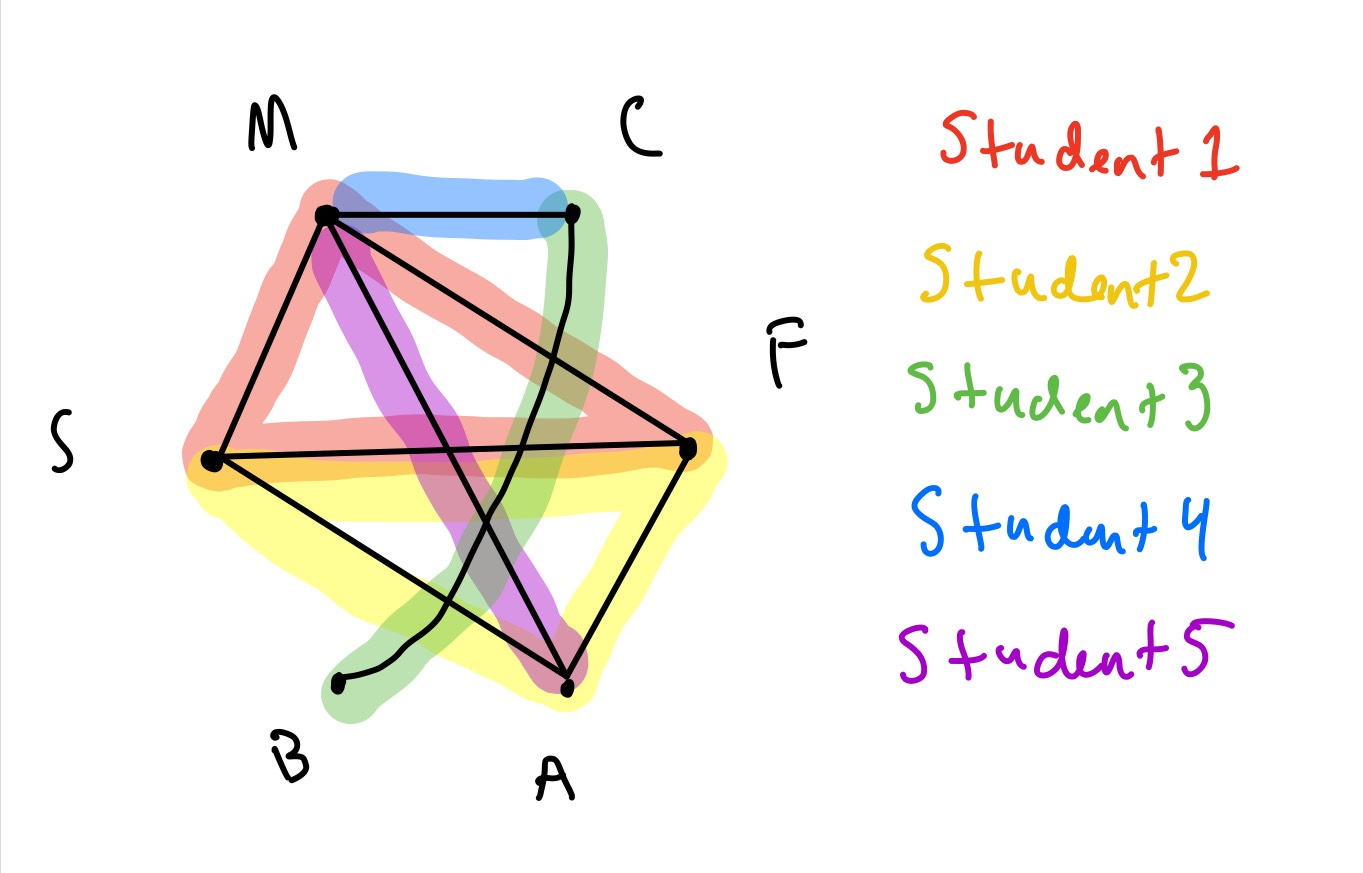
\includegraphics[width=11cm]{pics/final-conflicts.jpeg}
\end{center}

\begin{question}{}
How many timeslots do we need for these final exams? How can we pick which exams go in which timeslot?
\end{question}

Again, colorings of this graph correspond to conflict-free exam schedules. You can check that it's impossible to 3-color the graph (so we need more than 3 timeslots), but we can 4-color the graph as follows: 

\begin{center}
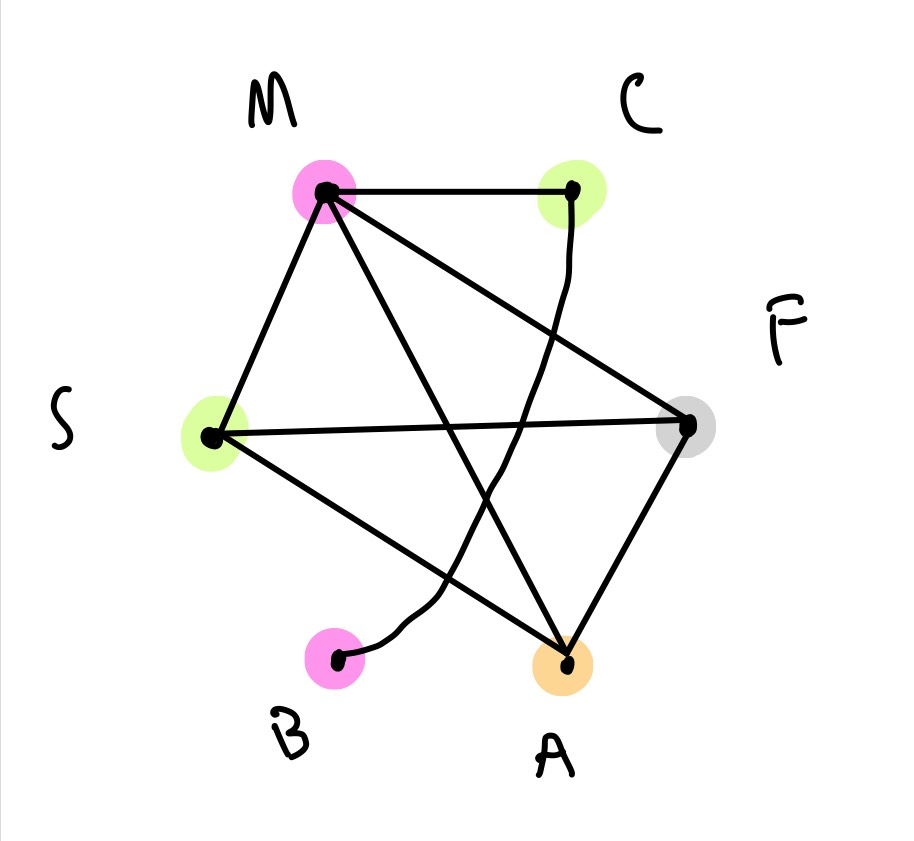
\includegraphics[width=5cm]{pics/final-coloring.jpeg}
\begin{tabular}{c|c}
 \multicolumn{2}{c}{Timeslots}\\
\hline
 Color & Vertices of that color \\
 \hline
 \hline
Hot pink & Math, Biology\\
 \hline
  Lime green & Computer science, Sociology \\
 \hline
 Grey & French \\
 \hline
 Orange & Anthropology
 \end{tabular}
 \end{center}
 
Hence we can have Math and Biology in the first timeslot, Computer science and Sociology in the second timeslot, French in the third timeslot, and Anthropology in the fourth timeslot.



%%%
\section{Chromatic polynomial of a graph}
%%%

The previous section was motivated by a more applied thinking about graphs. In this section, we would like to discuss what mathematicians care about.

In general, when mathematicians define a certain kind of object -- geometric shape, function, graph, set -- we then ask a question about how to classify these objects. For example, for sets, we can count the number of elements (which may be infinite), and if two sets have the same number of elements, then there is a bijection between them, in other words, we can identify their elements. After suitable identifications, we can start asking what are significant distinctions between the objects. For example, to each we can assign a number, like the chromatic number for a graph. These numbers are called \emph{invariants}.

For graphs, one invariant that is closely related to the chromatic number is the \emph{chromatic function}.

\begin{definition}
Let $G$ be a graph. Then we define the \emph{chromatic function} $P_G: \N \to \N$ by the following rule:
$P_G(n)=$ the number of colorings of the vertices of $G$ into $n$ colors.
\end{definition}

Let us compute some examples.

\begin{example}
Let first $G$ be the graph with one vertex and no edges, so $V = \{A\}$ and $E = \varnothing$. It looks like a dot. Given $n$ colors, we can color this dot in exactly $n$ ways, one for each choice of color, so $P_G(n) = n$.
\end{example}

\begin{example}
Let us go a few steps further and set $G$ to be the graph with 3 vertices and no edges, so $V = \{A,B,C\}$ and $E = \varnothing$. It looks like three dots. Given $n$ colors, we can color the vertex $A$ in $n$ ways. Then we are free to choose any color for $B$, since it is not connected to any other vertices, so for each of the first $n$ variants, we have $n$ variants in turn, which brings us to $n^2$ variants. Finally, the third vertex $C$ is not connected to any others, so we can color it  in $n$ ways independently of the previous choices. In total, it brings us to $P_G(n) = n^3$. 
\end{example}

\begin{exercise}
Generalize the previous two examples as follows: if $G$ is a graph with $v$ vertices and no edges, prove by induction that $P_G(n) = n^v$.
\end{exercise}

Let us now consider a more involved example -- graphs that have not just vertices, but also edges. You may have already guessed that graphs with loops (edges that begin and end in the same vertex) cannot be colored at all. Indeed, if you have a loop $AA$, definition of coloring tells us that the color of the vertex on the one side of $AA$ cannot be the same as color of the vertex on the other side... but oh no, it is the same vertex! So we can ignore graphs with loops because for them the problem of counting is trivial. Furthermore, if you have multiple edges that connect the two vertices, say $A$ and $B$, then each of the edges gives the same condition -- that $A$ and $B$ should be colored differently. So we can also ignore all but one edge between $A$ and $B$. To sum up, from now on we can only consider graphs that don't have loops, and each pair of vertices shares at most one edge.

\begin{definition}
    A \emph{simple graph} is one in which there is at most one edge joining a given 
    pair of vertices and there are no loops (i.e. edges joining a given vertex with itself).
\end{definition}


\begin{example}
Let us consider a graph with $v$ vertices that looks like a string, we will call this graph $A_v$.

Let us start with $v=5$ vertices and count the number of colorings of this graph into $n$ colors, that is we will calculate the value $P_{A_5}(n)$. We'll first color the leftmost vertex -- for this, we have $n$ choices of colors. But when we pick a color for the second vertex, we notice that one color -- the color of the first vertex -- is no longer available. So we now have $n-1$ choices. Similarly, the third vertex is connected to one vertex which is already colored, yielding $n-1$ choices again, and same for the fourth and fifth vertex. So altogether, we get the following result:
$$ P_{A_5}(n) = n(n-1)^4 \,.$$
\end{example}

\begin{exercise}
Guess a formula for $P_{A_v}(n)$ and prove it by induction.
\end{exercise}


\begin{example}
\label{ex:coloring_square}
Now let us consider the graph that can be drawn as a square, let's call it $G$:

\begin{center}
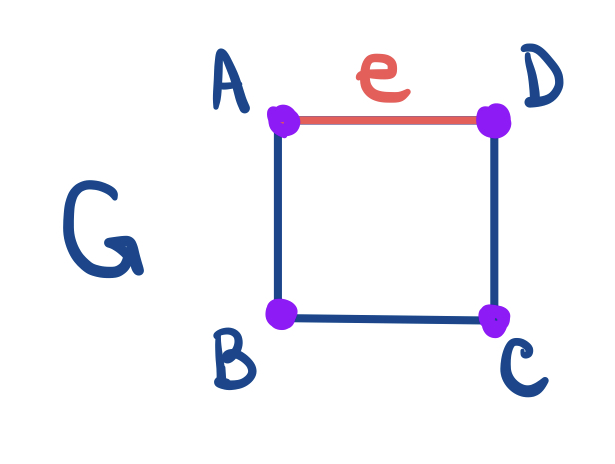
\includegraphics[width=3cm]{pics/coloring_square.jpg}
\end{center}

Its set of vertices is
$$ V = \{ A,B,C,D \}
,$$
and the set of edges is 
$$ E = \{AB,BC,CD,AD\}
.$$

We denote by $e$ the edge $AD$.

Now we can see how we can color this graph using, let's say, 4 colors. We will be coloring the vertices one after another and see which cases we encounter. There are 4 variants for the vertex $A$. For the next vertex, $B$, there are now three variants, because it is connected to one vertex that is already colored. So far, we have $4\cdot 3 = 12$ variants to color two first vertices.

Similarly, after $A$ and $B$ are colored, there are three variants to color $C$. However, we run into trouble now with $D$, because it is connected to both $A$ and $C$, and we don't know if they are the same color or different. Out of the three variants to color $C$, there is one case when $A$ and $C$ are of the same color -- in this case, we can choose out of three colors for $D$; and there are two cases when $A$ and $C$ have different colors -- then in each we can choose out of 2 colors to color $D$. In total, we have the following number of colorings:
$$ P_G(4) = 4 \cdot 3 \cdot (1 \cdot 3 + 2 \cdot 2) = 84
.$$
\end{example}

There is another approach to the same problem where you may choose to ignore the edge $e = AD$. If you delete this edge from $G$, you will get the graph $A_4$, and there we have less restrictions for coloring. In general, when you \emph{delete} $e$ from $G$, the result is denoted by $G-e$.

\begin{center}
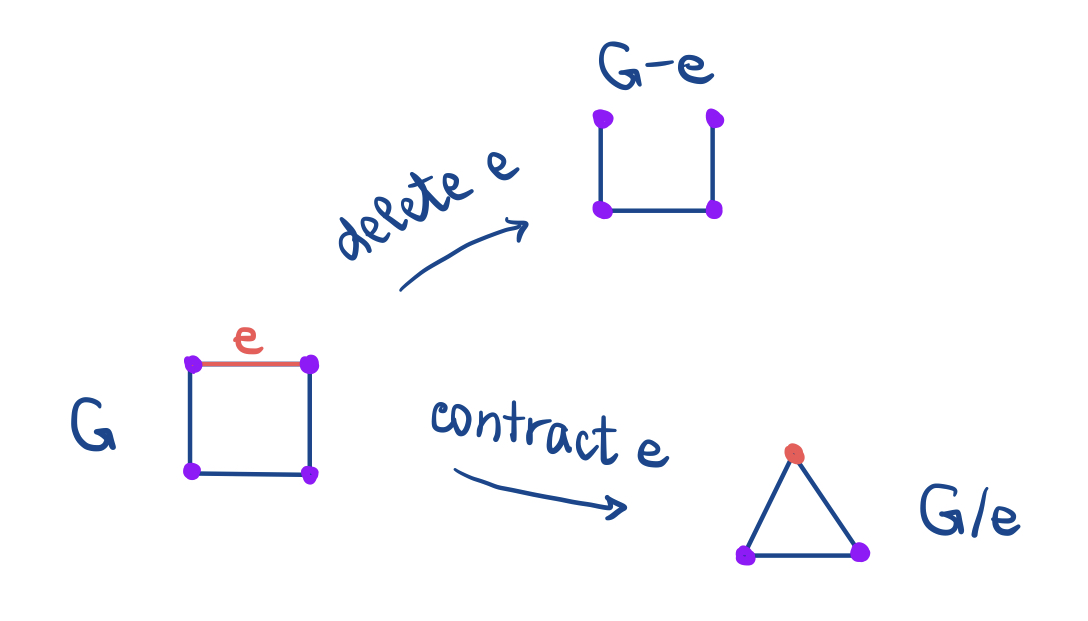
\includegraphics[width=7cm]{pics/coloring_square_deletecontract.jpg}
\end{center}

In fact, for each coloring of $G-e$, there are two cases: 
\begin{enumerate}
    \item Vertices of $e$ (in our case $A$ and $D$) have different colors. In this case, you can restore the edge $e$ and get a coloring of the original graph $G$.
    \item Vertices of $e$ have the same color. Then we can no longer draw an edge between them, because we cannot have an edge that connects vertices of the same color; however, we can glue these two vertices instead. This is called \emph{contracting} the edge $e$ of $G$.
\end{enumerate}

\begin{center}
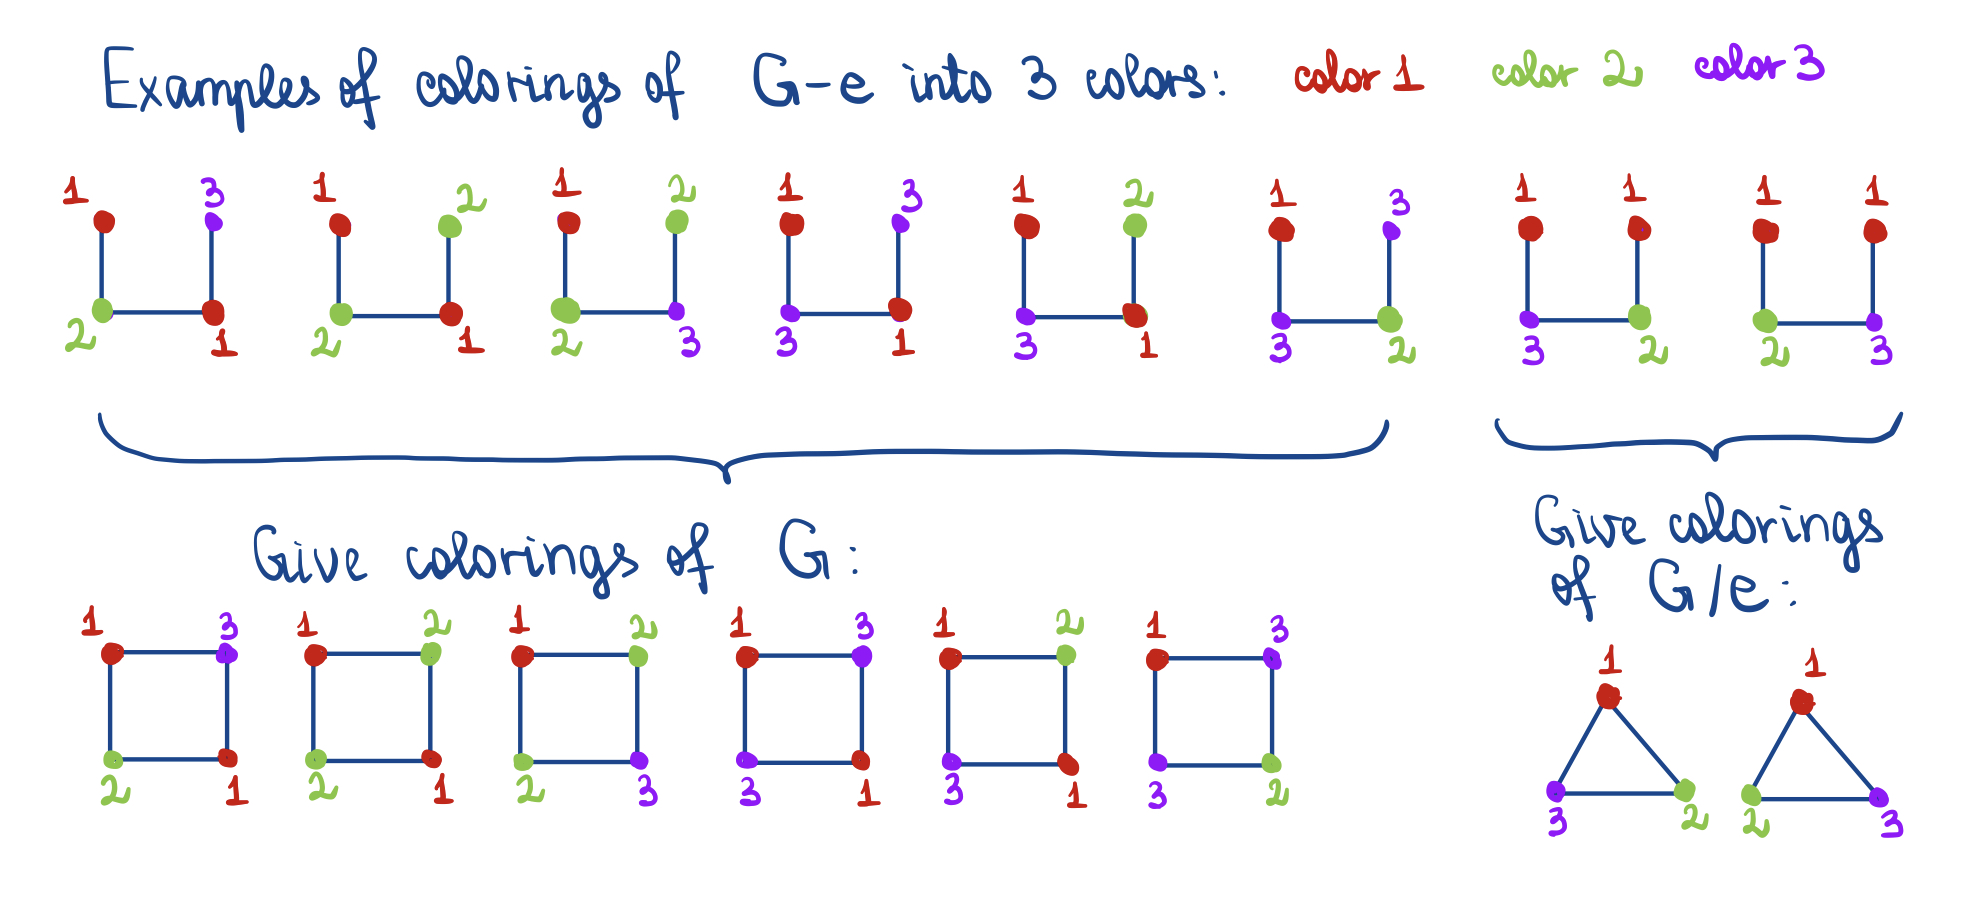
\includegraphics[width=12cm]{pics/coloring_square_cases.jpg}
\end{center}


The following is a cute theorem that generalizes the above observation. To prove it, you may use the same case-by-case analysis as we did for the square, as you may have already noticed that it didn't use the structure of $G$.

\begin{theorem}[Deletion-contraction formula]
   Let $G$ be a graph, and let $G-e$ and $G/e$, respectively, be the graphs obtained 
   from $G$ by deleting and contracting the edge $e$.
   Then
   \begin{equation*}
       P_G(n) = P_{G-e}(n) - P_{G/e}(n)\,.
   \end{equation*}
\end{theorem}

\begin{example}
Returning to the example with the square, denoted again by $G$, we can now compute $P_G(n)$ with the help of the new formula:
$$ P_G(n) = P_{A_4}(n) - P_{G/e}(n) = n(n-1)^3 - P_{G/e}(n)
.$$
Looking at the picture of $G/e$, one can compute $P_{G/e}(n)$: when we first color the vertex $A$, we have $n$ choices; for $B$, since it is connected to $A$, we have $n-1$ choices; and vertex $C$ is connected to $B$ as well as to $A$ (because we contracted $AD$, so $A$ and $D$ are now one vertex) -- so we have $n-2$ choices for $C$, because $A$ and $B$ are two different colors. In total, we have
$$P_{G/e}(n) = n(n-1)(n-2)
$$
colorings of $G/e$.

Finally, we plug in this result into $P_G(n)$:
\begin{equation*}
\begin{split}
    P_G(n) &= n(n-1)^3 - n(n-1)(n-2) = 
n(n-1) \left( (n-1)^2 - (n-2) \right) = \\
    &= n(n-1)(n^2 - 3n +3)
.
\end{split}    
\end{equation*}

We can check that this result recovers our calculation in Example \ref{ex:coloring_square} for $n=4$:
$$ P_G(4) = 4 \cdot 3 \cdot (16 - 12 + 3) = 84
.$$
    
\end{example}




\section{Euler characteristics}

Here is a little bit of magic. 
Close your eyes and start doodling without lifting your pencils.
Don't try too hard because we are going to do some math with your masterpiece.
Here's an example of what a doodling looks like.

\begin{figure}[htpb]
    \centering
    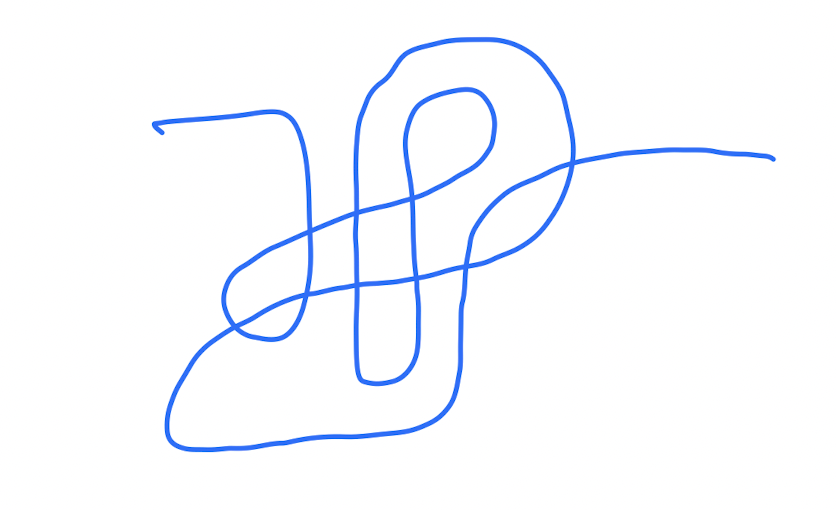
\includegraphics[width=0.4\linewidth]{Figures/doodle1}
    \caption{Doodling}%
    \label{fig:doodle1}
\end{figure}

Now, in order to do some math, please use a red pen to color all the intersections as well as the starting and ending points
in your masterpiece like the Figure~\ref{fig:doodle2}.

\begin{figure}[htpb]
    \centering
    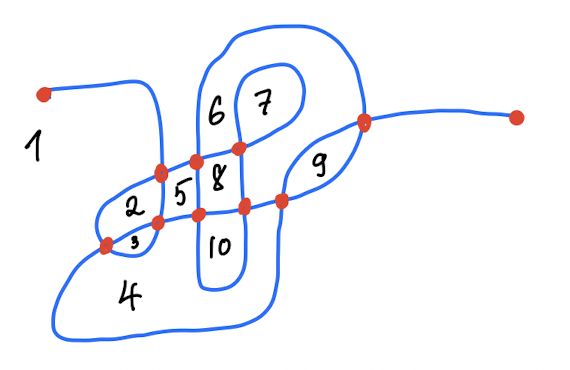
\includegraphics[width=0.4\linewidth]{Figures/doodle2}
    \caption{Color the intersections}%
    \label{fig:doodle2}
\end{figure}

Now, we have turned our doodling into a graph!
Let us count the number of vertices, number of edges and the number of 
regions this graph has divided our paper into (each region is the blank spaced enclosed
by some vertices and edges, just like countries and borders; we also count the area
not enclosed by anything one big region of its own).

Here are the counts for this graph.

\begin{itemize}
    \item Regions: 10
    \item Vertices: 11
    \item Edges: 19
\end{itemize}

Whatever you do, you should have the following relationship:
\begin{equation}
    \label{eq:euler}
    F + V - E = 2 \,,
\end{equation}
where $F$ stands for face (the regions), $V$ stands for vertices, $E$ stands for edges.

\begin{definition}
    The number $\cC(G) = F + V - E$ is called the Euler characteristics of a graph $G$.
\end{definition}

\begin{definition}[Spanning Tree]
   A spanning tree of a graph $G$ is a connected subgraph of $G$ 
   so that every pair of vertices is connected by exactly one path. 
\end{definition}

\begin{proposition}
    \label{t:spanning-tree}
   Every connected graph $G$ contains a spanning tree. 
\end{proposition}
We will not prove this proposition but use it to prove the following theorem.
\begin{theorem}
   The Euler characteristics of a connected planar graph is always 2. 
\end{theorem}

\begin{proof}
    Let $G$ be a connected graph.
    Let $T$ be a spanning tree of $G$ given by Theorem~\ref{t:spanning-tree}.
    For a tree $T$, the number of edges is always one less than the number of vertices, i.e., $V = E + 1$. Because there are no cycles in a tree, the number of faces is $F = 1$.
    So $\cC(T) = 2$. To obtain $G$ from $T$, 
    we add more edges. Each time we add an edge, we add a new face. Thus, the Euler characteristics doesn't change after we add the edges to make $T$ become $G$.
    As a consequence, $\cC(G) = 2$.
\end{proof}


We will have to define what a region means for non-planar graphs (which is out
of the scope of this class) but once we define that, 
we can prove that the Euler characteristics of non-planar graphs are not 2.



Let us use the Euler characteristics to show a very surprising fact about
Platonic solids.

\begin{definition}[Regular polygon]
   A \emph{regular polygon} is a polygon that has all angles equal and all sides equal. 
\end{definition}

\begin{definition}[Platnoic solids]
   A  \emph{Platonic solid} is a 3-dimensional shape such that
   \begin{itemize}
       \item Each face is the same regular polygon.
       \item The same number of polygons meet at each vertex.
   \end{itemize}
\end{definition}

\begin{theorem}
   There are only 5 Platonic solids. 
\end{theorem}

\begin{proof}
    Suppose we have a Platonic solid.
    Let $F$ be the number of faces, $E$ be the number of edges, $V$ be the number
    of vertices of the solid.

    Let us observe a few things.
    First, on each face, the number of edges and vertices is the same.
    Let $N$ be the number of edge and vertices on \emph{each} face. 
    Let $D$ be the degree of each vertex.

    Second, since each edge belongs to two different faces and each 
    edge also joins two vertices,
    \begin{equation*}
        NF = 2E = DV \,.
    \end{equation*}

    Note that we can redraw the faces, vertices and edges of a Platonic solid
    into a plane graph (you should try a few!).
    By the Euler's characteristics theorem,
    \begin{equation*}
        2 = V + F - E   = V + \frac{DV}{N} - \frac{DV}{2} \,. 
    \end{equation*}
    Rearrange terms, we have
    \begin{equation*}
        V(2N + 2D - ND) = 4N \,.
    \end{equation*}
    It must be true then that $2N + 2D - ND > 0$ as $V, N >0$.
    This means $(N- 2)(D-2) <4$ and there are only 5 possibilities for $N, D >0$,

    \begin{equation*}
        (N,D) = \begin{dcases}
            (3,3) \quad \text{ tetrahedron}\,, \\
            (3,4) \quad \text{ cube}\,, \\
            (4,3) \quad \text{ octahedron}\,, \\
            (3,5) \quad \text{ dodecahedron}\,, \\
            (5,3) \quad \text{ icosahedron} \,.
        \end{dcases}
    \end{equation*}
    This is our claim!
\end{proof}


